\makeatletter\def\input@path{{../template/vsp-beamer}{../template/minimus}}\makeatother

\documentclass[red,tutorial,sectionpages,shtu]{vsp-beamer}

\graphicspath{{image/}{../template/vsp-beamer/assets/}}

\usepackage{minimus-section}
\usepackage{minimus-text}
\usepackage{minimus-math}
\usepackage{minimus-float}
\usepackage{minimus-code}
\usepackage{minimus-colorbox}
\usepackage{minimus-reference}
\usepackage{tikz}
\usetikzlibrary{arrows.meta,positioning,calc}
\lstset{basicstyle=\ttfamily\footnotesize,numberstyle=\tiny\color{gray},breaklines=true}

\title{CS100 Recitation 4}
\subtitle{GDB、Sanitizer与C语言代码调试}
\VSPsetspeaker{Wenjie Liu}{liuwj2026@shanghaitech.edu.cn}
\VSPsetupfootline{CS100 Recitation 4}{Fall 2026}{Wenjie Liu}

\begin{document}

\VSPtitleframe

\begin{frame}{成绩统计：完整代码（调试用错误版）}
    \lstset{basicstyle=\ttfamily\fontsize{7.5}{8.8}\selectfont,
        numberstyle=\fontsize{4.8}{5.5}\selectfont\color{gray},xleftmargin=6pt}
    \begin{columns}[T]
        \begin{column}{0.48\textwidth}
            \begin{Code}*{c}
                \lstinputlisting[firstline=1,lastline=14,firstnumber=1]{code/gdb/grades.c}
            \end{Code}
        \end{column}
        \begin{column}{0.48\textwidth}
            \begin{Code}*{c}
                \lstinputlisting[firstline=15,firstnumber=15,lastline=28]{code/gdb/grades.c}
            \end{Code}
        \end{column}
    \end{columns}
    \note{成绩统计示例已改写为C，读取成绩时直接累计，不使用容器或动态内存。代码读取人数n和n个成绩，计算及格成绩平均值；人数统计的score > 60与求和条件不一致，保留该错误供调试观察。}
\end{frame}

\begin{frame}{成绩统计：程序运行了，结果就正确吗？}
    \begin{columns}[c]
        \begin{column}{0.56\textwidth}
            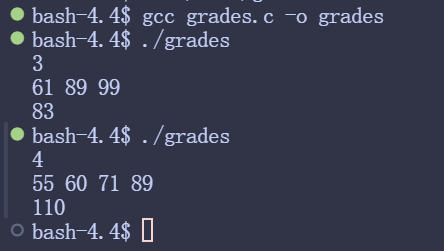
\includegraphics[width=\linewidth,height=0.73\textheight,keepaspectratio]{gradeserro.png}
        \end{column}
        \begin{column}{0.40\textwidth}
            \alert{第一组：61、89、99}
            \par 预期平均值83，输出83。
            \medskip

            \alert{第二组：55、60、71、89}
            \par 及格成绩为60、71、89。
            \par 预期$220/3\approx73.3333$，
            \par 实际输出\alert{110}。
            \medskip

            同一段代码，为什么一组正确，另一组错误？
        \end{column}
    \end{columns}
    \note{结合上一页完整代码，先让学生手算两组结果，再观察错误原因。截图来自用户提供的image/gradeserro.png，不对截图内容做修改。}
\end{frame}

\begin{frame}{目录}
    \tableofcontents[hideallsubsections]
    \medskip
    \small 后续命令统一在提交包的\texttt{r4/}目录执行；课前运行\texttt{make demos}构建演示程序。
\end{frame}

\section{程序出错之后，从哪里开始？}

\begin{frame}{HW1：完整代码（调试用错误版）}
    \small 依据HW1 P3要求编写的课堂调试变体：读整数至0，输出总和与最大值。
    \lstset{basicstyle=\ttfamily\fontsize{7.5}{8.8}\selectfont,
        numberstyle=\fontsize{4.8}{5.5}\selectfont\color{gray},xleftmargin=6pt}
    \begin{columns}[T]
        \begin{column}{0.48\textwidth}
            \begin{Code}*{c}
                \lstinputlisting[firstline=1,lastline=14,firstnumber=1]{code/homework/hw1-p3.c}
            \end{Code}
        \end{column}
        \begin{column}{0.48\textwidth}
            \begin{Code}*{c}
                \lstinputlisting[firstline=15,firstnumber=15,lastline=30]{code/homework/hw1-p3.c}
            \end{Code}
        \end{column}
    \end{columns}
    \note{完整展示现有HW1错误版，不使用数组或动态内存。先让学生预测程序输出，再用下一页的小输入检验。错误位于更新最大值时传入了sum而不是x；后续用GDB观察调用者和被调用函数中的变量。现场演示直接使用code/homework/hw1-p3.c。}
\end{frame}

\begin{frame}{HW1：编译通过，然后呢？}
    P3的starter要求：读整数，遇到0结束，输出\alert{总和与最大值}；不用数组或动态内存。
    \begin{columns}[T]
        \begin{column}{0.52\textwidth}
            \begin{block}{课堂运行截图}
                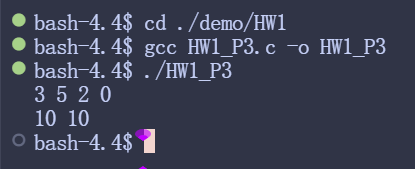
\includegraphics[width=\linewidth,height=0.42\textheight,keepaspectratio]{HW1_P3.png}
            \end{block}
            输入：\texttt{3 5 2 0}。\par
            0是结束标记，不是待统计的数据。
        \end{column}
        \begin{column}{0.44\textwidth}
            \begin{itemize}
                \item 总和：$3+5+2=10$。
                \item 最大值：5。
                \item 预期输出：\texttt{10 5}。
                \item 错误版输出：\alert{\texttt{10 10}}。
            \end{itemize}
        \end{column}
    \end{columns}
    \medskip
    \alert{能编译、能运行，不代表实现了需求。}先用小输入找出差异。
    \note{截图使用用户提供的image/HW1_P3.png，展示编译成功后输入3 5 2 0却输出10 10的现象。先对照手算结果，再进入后续调试流程。}
\end{frame}

\begin{frame}{先说清楚：错在哪里？}
    \begin{center}
        \renewcommand{\arraystretch}{1.4}
        \begin{tabular}{p{0.23\linewidth}p{0.60\linewidth}}
            \textbf{现象} & \textbf{第一步要收集什么？} \\
            编译或链接失败 & 完整命令、第一条诊断、对应源码。 \\
            运行崩溃 & 能复现的输入、信号、调用栈。 \\
            输出错误 & 明确的预期结果、一个小反例。 \\
            一直不结束 & 输入是否读完、程序停在哪个循环或调用。
        \end{tabular}
    \end{center}
    \medskip
    “我的程序有问题”还不够。先补全：\alert{输入是什么？应该怎样？实际怎样？}
\end{frame}

\begin{frame}{一次只验证一个猜想}
    对于输出\texttt{10 10}的HW1课堂变体，先问：
    \begin{enumerate}
        \item 是否依次读到了3、5、2，并在0处停止？
        \item 每轮结束后，总和是否依次为3、8、10？
        \item 最大值是否依次为3、5、5？
        \item 传给更新最大值函数的，是当前输入，还是别的量？
    \end{enumerate}
    \medskip
    \begin{vspquotered}{让猜想可以被验证}
        写下“这里应该是多少”，再观察“这里实际是多少”。\par
        保留失败输入，每次修改后重新运行。
    \end{vspquotered}
\end{frame}

\begin{frame}{从复现到验证：工具分别帮什么忙？}
    \begin{center}
        \begin{tikzpicture}[node distance=0.27cm,>=Stealth,
            every node/.style={font=\small},
            stage/.style={draw=VSPPrimary,rounded corners,align=center,
                minimum width=1.85cm,minimum height=0.8cm}]
            \node[stage] (a) {复现错误};
            \node[stage,right=of a] (b) {缩小范围};
            \node[stage,right=of b] (c) {观察状态};
            \node[stage,right=of c] (d) {解释原因};
            \node[stage,right=of d] (e) {修复验证};
            \draw[->] (a)--(b); \draw[->] (b)--(c);
            \draw[->] (c)--(d); \draw[->] (d)--(e);
        \end{tikzpicture}
    \end{center}
    \begin{itemize}
        \item \alert{编译警告}：编译时发现可疑写法；逐条阅读。
        \item \alert{日志与断言}：记录关键状态，检查必须成立的条件。
        \item \alert{GDB}：观察变量、执行位置与调用栈。
        \item \alert{Sanitizer}：在运行时检查特定类别的非法行为。
    \end{itemize}
    工具提供线索；预期结果与原因解释，需要你来确定。
    \note{本节约8分钟。先让学生手算总和10与最大值5，再预测每轮的中间状态。}
\end{frame}

\section{GDB：让程序停下来看看}

\begin{frame}{GDB是什么？}
    \alert{GDB（GNU Debugger）}是GNU项目的调试器，本课使用它调试C语言编写的程序。
    \medskip
    \begin{itemize}
        \item \alert{启动程序}：指定参数和输入，复现出错的运行过程。
        \item \alert{暂停执行}：在某个位置、条件成立或变量改变时停下来。
        \item \alert{查看现场}：观察变量、源码位置和函数调用关系。
        \item \alert{控制执行}：逐步运行，找到实际行为第一次偏离预期的位置。
    \end{itemize}
    \medskip
    \begin{vspquotered}{从源码到调试}
        \texttt{gcc}将C源码编译为可执行程序；GDB加载并调试这个程序。\par
        VSCode可以通过扩展调用编译器与调试器，提供图形化操作界面。
    \end{vspquotered}
    \small 调试信息帮助GDB显示源码行号与变量；后面将介绍编译参数\texttt{-g}。
\end{frame}

\begin{frame}{GDB与GCC有什么区别？}
    \alert{GCC负责把源码编译成程序，GDB负责观察和控制程序的运行。}
    \medskip
    \begin{columns}[T]
        \begin{column}{0.51\textwidth}
            \small
            \begin{itemize}
                \item \texttt{gcc}读取C源码，编译、链接成可执行程序。
                \item \texttt{gdb}加载可执行程序，设置断点、查看变量、单步执行。
            \end{itemize}
            \medskip
            在终端中\alert{先编译，再启动调试}：
            \lstset{basicstyle=\ttfamily\fontsize{7.2}{8.7}\selectfont,
                numberstyle=\fontsize{4.8}{5.5}\selectfont\color{gray},
                xleftmargin=6pt,breakatwhitespace=true}
            \begin{Code}*{bash}
                \lstinputlisting{code/commands/compile-and-debug.sh}
            \end{Code}
            修改源码后，需要先重新编译。
        \end{column}
        \begin{column}{0.45\textwidth}
            \small
            \renewcommand{\arraystretch}{1.25}
            \begin{tabular}{@{}p{0.27\linewidth}p{0.65\linewidth}@{}}
                \textbf{选项} & \textbf{含义} \\
                \texttt{-g} & 生成调试信息，便于GDB定位源码和变量。 \\
                \texttt{-O0} & 关闭优化，便于逐行调试。 \\
                \texttt{-Wall} & 开启一组常用编译警告。 \\
                \texttt{-Wextra} & 开启额外的编译警告。 \\
                \texttt{-Wpedantic} & 提示部分不符合所选ISO C标准的写法。 \\
                \texttt{-Werror} & 将警告视为错误，有警告时编译失败。
            \end{tabular}
        \end{column}
    \end{columns}
    \medskip
    \footnotesize \texttt{-O0}中的O是字母、0是数字；\texttt{-Wall}并非开启全部警告。
    \note{补充六个GCC选项的含义。-g生成调试信息；-O0便于本课按源码逐行观察。-Wall与-Wextra启用不同的警告集合，-Wpedantic依据-std=c17检查部分标准符合性，-Werror将警告提升为错误。提醒不要将-Werror拼成-Werro。}
\end{frame}

\begin{frame}{安装GDB：Ubuntu／WSL}
    在\alert{Ubuntu／WSL的Ubuntu终端}执行以下命令，需要当前账号拥有sudo权限：
    \begin{Code}*{bash}
        \lstinputlisting{code/commands/install.sh}
    \end{Code}
    \begin{columns}[c]
        \begin{column}{0.62\textwidth}
            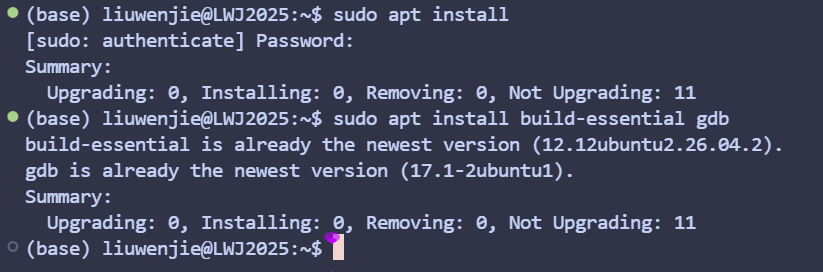
\includegraphics[width=\linewidth,height=0.40\textheight,keepaspectratio]{gdb_install.png}
        \end{column}
        \begin{column}{0.34\textwidth}
            \small
            \begin{itemize}
                \item \texttt{apt update}：更新软件包索引。
                \item \texttt{build-essential}：GCC、Make等构建工具。
                \item \texttt{gdb}：GDB调试器。
            \end{itemize}
        \end{column}
    \end{columns}
    \medskip
    \small 截图中的\texttt{is already the newest version}表示相应工具已安装。
    \par 共享服务器可能使用其他发行版或没有sudo权限，安装前先确认环境。
    \note{展示用户提供的image/gdb_install.png。截图显示build-essential与gdb已为该环境中的最新可用版本；版本号以实际环境为准。Windows用户先进入WSL的Ubuntu环境。}
\end{frame}

\begin{frame}{没有sudo权限时怎么使用GDB？}
    \texttt{is not in the sudoers file}表示当前账号没有sudo权限。
    \begin{itemize}
        \item 在共享服务器上，使用管理员提供的工具，或已准备好的用户目录工具。
        \item 本项目当前演示机是\alert{RHEL 8.10}；Ubuntu的\texttt{apt}安装命令不适用。
    \end{itemize}
    \medskip
    当前工作区已准备好本地GDB与运行库，可以在Bash中执行：
    \begin{Code}*{bash}
        \lstinputlisting{code/commands/use-local-tools.sh}
    \end{Code}
    \small 这里加载的是本工作区已有工具。每次打开新终端需重新加载；清理\texttt{build/}后需重新准备这些工具。其他服务器的工具路径以管理员说明为准。
\end{frame}

\begin{frame}{安装完成后，如何验证？}
    \begin{columns}[T]
        \begin{column}{0.48\textwidth}
            在\alert{终端}中依次执行：
            \begin{Code}*{bash}
                \lstinputlisting{code/commands/verify-install.sh}
            \end{Code}
            \texttt{command -v}显示GDB路径；\par
            \texttt{--version}显示版本信息。
        \end{column}
        \begin{column}{0.48\textwidth}
            出现\alert{\texttt{(gdb)}}提示符后输入：
            \begin{Code}*{plain}
                \lstinputlisting{code/commands/verify-install.gdb}
            \end{Code}
            \texttt{help}显示命令帮助；\par
            \texttt{quit}退出并回到终端。
        \end{column}
    \end{columns}
    \medskip
    \begin{vspquotered}{验证成功的标志}
        能找到路径、显示版本，并进入GDB执行\texttt{help}，说明工具已可启动。\par
        若提示\texttt{command not found}，先检查安装位置或是否加载了本地工具环境。
    \end{vspquotered}
\end{frame}

\begin{frame}{这四行命令分别验证什么？}
    \begin{center}
        \renewcommand{\arraystretch}{1.3}
        \begin{tabular}{p{0.25\linewidth}p{0.65\linewidth}}
            \textbf{终端命令} & \textbf{含义与成功时的现象} \\
            \texttt{command -v gdb} &
                让Shell查找\texttt{gdb}命令，检查当前终端能否找到它；通常输出可执行文件路径。 \\
            \texttt{gdb --version} &
                显示GDB的版本信息并退出，确认调试器可以运行，也方便记录调试环境。 \\
            \texttt{gcc --version} &
                显示GCC的版本信息并退出，确认C编译器可以运行；后面用它编译示例源码。 \\
            \texttt{gdb -q} &
                以安静模式启动GDB，省略欢迎语和版权信息；出现\texttt{(gdb)}后即可输入调试命令。
        \end{tabular}
    \end{center}
    \medskip
    \texttt{-q}中的q表示\alert{quiet}；进入GDB后用\texttt{help}查看帮助，用\texttt{quit}退出。
    \par\small 工具已经安装但终端找不到时，检查\texttt{PATH}，或重新加载本地工具环境。
\end{frame}

\begin{frame}{安装验证：路径、版本与交互界面}
    \begin{columns}[T]
        \begin{column}{0.48\textwidth}
            \alert{查找路径、查看版本}
            \par\medskip
            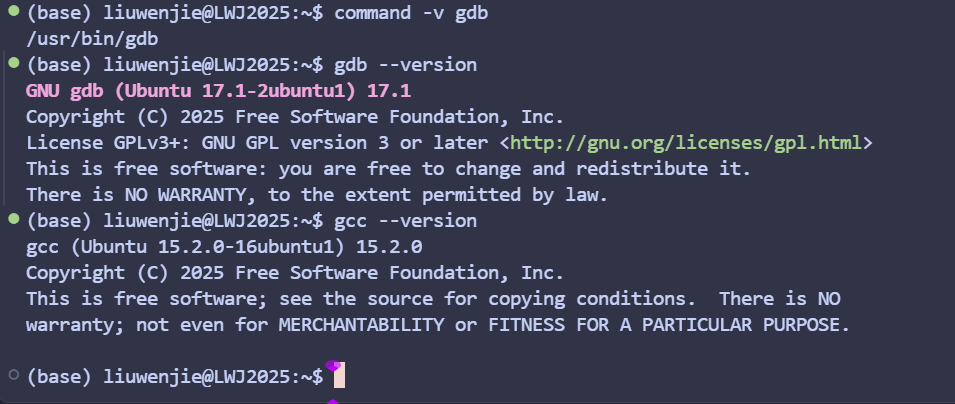
\includegraphics[width=\linewidth,height=0.64\textheight,keepaspectratio]{gdb_version.png}
            \par\medskip
            \small 显示GDB路径，以及GDB、GCC的版本信息。
        \end{column}
        \begin{column}{0.48\textwidth}
            \alert{启动GDB、查看帮助、退出}
            \par\medskip
            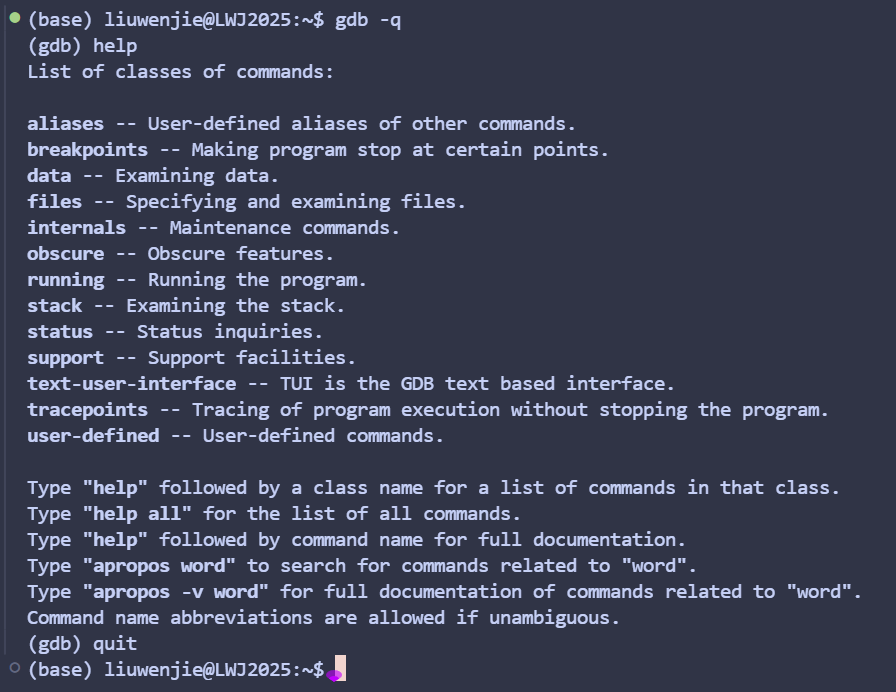
\includegraphics[width=\linewidth,height=0.64\textheight,keepaspectratio]{gdb-q.png}
            \par\small \texttt{gdb -q}进入，\texttt{help}查看帮助，\texttt{quit}退出。
        \end{column}
    \end{columns}
    \note{使用用户提供的image/gdb_version.png与image/gdb-q.png，分别展示前三条安装验证命令的输出和第四条命令的交互过程。版本号与路径取决于实际安装环境，不要求与截图一致。}
\end{frame}

\begin{frame}{GDB常用命令速查}
    \begin{center}
        \renewcommand{\arraystretch}{1.0}
        \begin{tabular}{lll}
            \textbf{命令示例} & \textbf{常用缩写} & \textbf{作用} \\
            \texttt{run} & \texttt{r} & 启动或重新运行程序 \\
            \texttt{break main} & \texttt{b main} & 在main函数设置断点 \\
            \texttt{continue} & \texttt{c} & 继续运行 \\
            \texttt{next} & \texttt{n} & 在当前调用层级单步执行 \\
            \texttt{step} & \texttt{s} & 单步执行，尝试进入函数 \\
            \texttt{finish} & \texttt{fin} & 运行到当前选定函数返回 \\
            \texttt{print value} & \texttt{p value} & 查看变量或表达式的值 \\
            \texttt{list} & \texttt{l} & 查看源码 \\
            \texttt{backtrace} & \texttt{bt} & 查看调用栈 \\
            \texttt{help break} & \texttt{h break} & 查看某条命令的帮助 \\
            \texttt{quit} & \texttt{q} & 退出GDB
        \end{tabular}
    \end{center}
    \small 这些命令在\texttt{(gdb)}中输入；终端中的\texttt{gdb ./程序}用于启动调试器。
\end{frame}

\begin{frame}{让编译结果适合调试}
    \begin{Code}*{bash}
        \lstinputlisting{code/commands/build-debug.sh}
    \end{Code}
    \begin{itemize}
        \item \texttt{-std=c17}：显式指定本课使用的C17语言标准。
        \item \texttt{-g}：加入调试信息；\texttt{-O0}：本次演示关闭优化，便于逐行观察。
        \item \texttt{-Wall -Wextra -Wpedantic}：开启常用编译警告。
        \item 修改源码后\alert{重新编译}，确认正在调试的是新生成的程序。
    \end{itemize}
    \small 优化会改变源码与机器指令的对应关系；出现\texttt{optimized out}时检查构建参数。
\end{frame}

\begin{frame}{HW1：先看调用者与辅助函数}
    \begin{columns}[T]
        \begin{column}{0.52\textwidth}
            \alert{主循环中的调用：}
            \begin{Code}*{c}
                \lstinputlisting[firstline=18,lastline=24,firstnumber=18]{code/homework/hw1-p3.c}
            \end{Code}
        \end{column}
        \begin{column}{0.44\textwidth}
            \alert{更新最大值：}
            \begin{Code}*{c}
                \lstinputlisting[firstline=4,lastline=10,firstnumber=4]{code/homework/hw1-p3.c}
            \end{Code}
        \end{column}
    \end{columns}
    \medskip
    处理输入5时，\texttt{x == 5}、\texttt{sum == 8}。\par
    \alert{传入辅助函数的value应该是多少？实际又是多少？}
\end{frame}

\begin{frame}{先把失败输入固定下来}
    \begin{itemize}
        \item 输入文件：\texttt{code/input/sum-max.txt}，内容为\texttt{3 5 2 0}。
        \item 正常运行：\texttt{./build/demo/hw1-p3 < code/input/sum-max.txt}。
        \item 预期\texttt{10 5}，实际\texttt{10 10}；保留这个反例。
    \end{itemize}
    \medskip
    \begin{vspquotered}{下一步要验证的猜想}
        总和正确，但更新最大值时可能比较了错误的数据。\par
        观察调用者的\texttt{x / sum}与被调用函数的\texttt{value / result}。
    \end{vspquotered}
    \medskip
    \alert{小输入可以手算，也方便逐步跟踪。}
\end{frame}

\begin{frame}{第一次启动GDB}
    在终端启动调试器：
    \begin{Code}*{bash}
        \lstinputlisting{code/commands/start-gdb.sh}
    \end{Code}
    进入\texttt{(gdb)}提示符后输入：
    \begin{Code}*{plain}
        \lstinputlisting[firstline=1,lastline=2,firstnumber=1]{code/commands/basic.gdb}
    \end{Code}
    \begin{itemize}
        \item \texttt{break updateMaximum}：在更新最大值的函数设置断点。
        \item \texttt{run < ...}：使用同一份输入启动程序。
        \item 程序停住后，GDB显示当前源码位置。
    \end{itemize}
\end{frame}

\begin{frame}{HW1：从断点现场定位传参错误}
    \begin{columns}[c]
        \begin{column}{0.54\textwidth}
            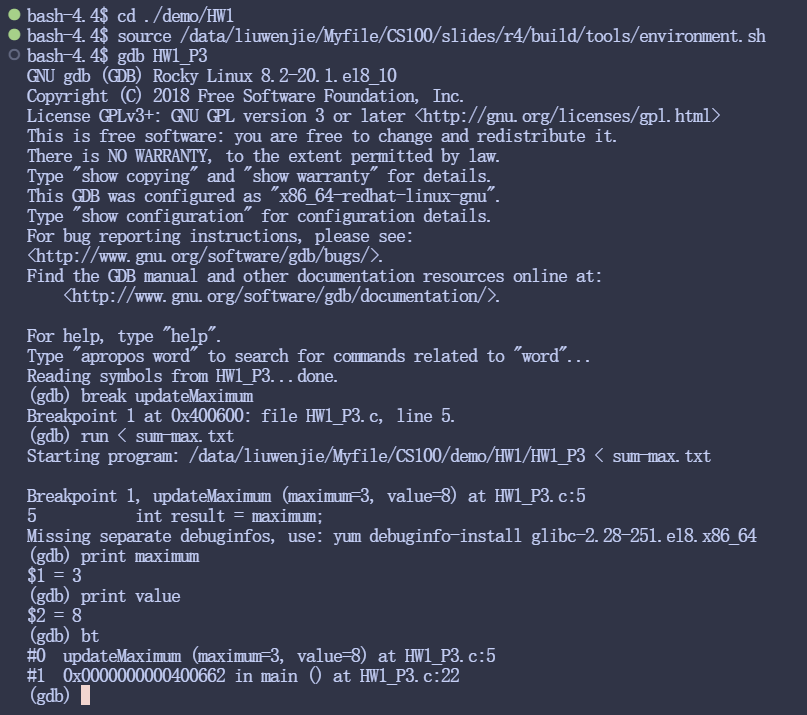
\includegraphics[width=\linewidth,height=0.80\textheight,keepaspectratio]{HW1_P3GDB.png}
        \end{column}
        \begin{column}{0.42\textwidth}
            \small
            \alert{断点已命中，检查传入的数据}
            \begin{itemize}
                \item \texttt{maximum = 3}：此前读到的最大值，符合预期。
                \item \texttt{value = 8}：当前输入是5，函数却收到了累计总和$3+5=8$。
                \item \texttt{bt}：当前在\texttt{updateMaximum}，调用来自\texttt{main}第22行。
            \end{itemize}
            \medskip
            \alert{检查调用处：将sum改为x}
            \par\texttt{updateMaximum(maximum, x)}
            \medskip

            \footnotesize 当前停在第5行，\texttt{result}尚未初始化；先执行\texttt{next}再查看它。
        \end{column}
    \end{columns}
    \note{截图使用image/HW1_P3GDB.png。第一次调用发生在读入5之后，maximum=3、sum=8；截图直接显示传入value=8，bt给出main第22行这一调用位置。可进一步frame 1、print x、print sum验证，再修复调用并重新编译，输入3 5 2 0应输出10 5。截图的系统库debuginfo提示不妨碍本例查看自己的源码和变量。}
\end{frame}

\begin{frame}{断点：只在你关心的位置停下来}
    \begin{center}
        \renewcommand{\arraystretch}{1.35}
        \begin{tabular}{ll}
            \textbf{命令} & \textbf{作用} \\
            \texttt{break updateMaximum} & 在函数入口设置断点 \\
            \texttt{break code/homework/hw1-p3.c:22} & 在指定文件行设置断点 \\
            \texttt{info breakpoints} & 查看断点编号与位置 \\
            \texttt{disable 1} / \texttt{enable 1} & 禁用／启用编号1的断点 \\
            \texttt{delete 1} & 删除编号1的断点 \\
            \texttt{continue} & 继续执行，直到再次停止
        \end{tabular}
    \end{center}
    \medskip
    \alert{当前行通常是即将执行的源码行。}读取变量时，要留意该行是否已经执行。
\end{frame}

\begin{frame}{观察变量：实际值符合预期吗？}
    在辅助函数中、\texttt{result}初始化后停住，再使用：
    \begin{Code}*{plain}
        \lstinputlisting{code/commands/inspect.gdb}
    \end{Code}
    \begin{columns}[c]
        \begin{column}{0.65\textwidth}
            \begin{itemize}
                \item \texttt{print}（\texttt{p}）：这一次查看一个变量或表达式。
                \item \texttt{display}：以后每次停止时自动显示表达式。
                \item \texttt{info locals}：查看当前栈帧中的局部变量。
            \end{itemize}
        \end{column}
        \begin{column}{0.29\textwidth}
            \centering
            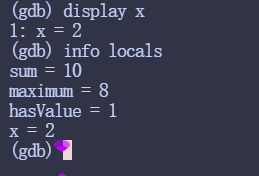
\includegraphics[width=\linewidth,height=0.30\textheight,keepaspectratio]{info.png}
            \par\scriptsize 截图：\texttt{main}中的局部变量。
        \end{column}
    \end{columns}
    \medskip
    变量存在\alert{作用域}；查看调用者的\texttt{x}和\texttt{sum}时，先切换到对应栈帧。
    \note{右侧使用image/info.png，展示main中display x与info locals的输出。截图属于第三个输入2的现场，x=2、sum=10、maximum=8；与上方辅助函数中的result示例处于不同的栈帧。}
\end{frame}

\begin{frame}{next、step与finish：函数调用处怎么走？}
    \begin{center}
        \begin{tikzpicture}[>=Stealth,node distance=0.9cm,
            box/.style={draw=VSPPrimary,rounded corners,align=left,
            inner sep=7pt,font=\small\ttfamily}]
            \node[box] (main) {main()\\\quad updateMaximum(maximum, sum);\\\quad print result;};
            \node[box,right=of main] (fn) {updateMaximum()\\\quad compare value;\\\quad return result;};
            \draw[->,thick] (main.north east) to[bend left=15]
                node[above,font=\small] {step：进入函数} (fn.north west);
            \draw[->,thick] (fn.south west) to[bend left=15]
                node[below,font=\small] {finish：运行至返回} (main.south east);
        \end{tikzpicture}
    \end{center}
    \begin{itemize}
        \item \texttt{next}（\texttt{n}）：在当前调用层级向前走，通常跨过函数调用。
        \item \texttt{step}（\texttt{s}）：尝试进入有源码调试信息的被调用函数。
        \item \texttt{finish}：运行到当前选定函数返回之后。
    \end{itemize}
    \small 遇到断点或信号可能提前停止。进入标准库内部时，可用\texttt{finish}返回。
\end{frame}

\begin{frame}{HW1现场：step、next与finish分别做了什么？}
    \begin{columns}[c]
        \begin{column}{0.54\textwidth}
            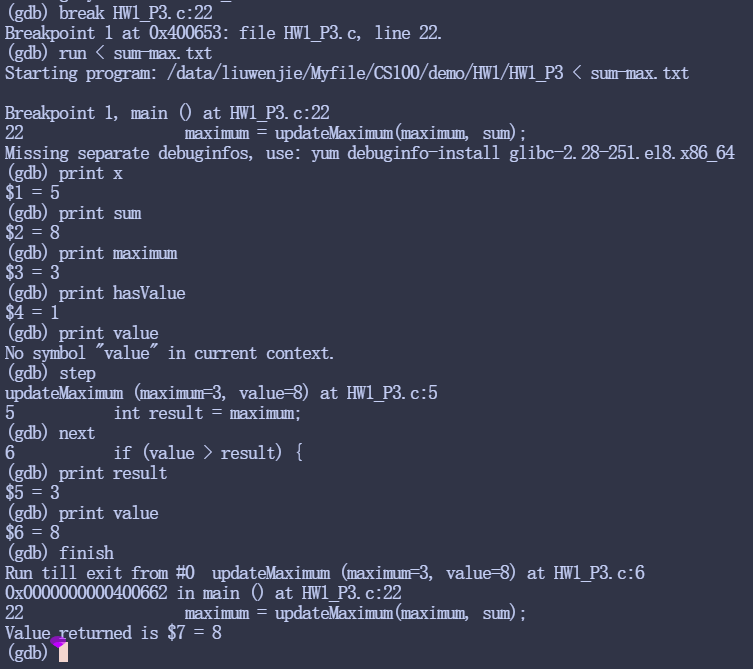
\includegraphics[width=\linewidth,height=0.80\textheight,keepaspectratio]{step_next_finish.png}
        \end{column}
        \begin{column}{0.42\textwidth}
            \small
            \begin{enumerate}
                \item \alert{step：进入函数。}\par
                    从\texttt{main}第22行进入\texttt{updateMaximum}第5行，收到\texttt{maximum=3, value=8}。
                \item \alert{next：执行初始化。}\par
                    执行第5行后停在第6行；此时\texttt{result=3}，\texttt{value=8}。
                \item \alert{finish：运行到函数返回。}\par
                    执行后续比较与返回，回到\texttt{main}，显示返回值\alert{8}。
            \end{enumerate}
            \medskip
            \footnotesize 若在第22行直接用\texttt{next}，则跨过这次调用。截图中\texttt{finish}后仍显示第22行，可再\texttt{next}完成赋值并查看\texttt{maximum}。
            \par\medskip
            \texttt{value}是辅助函数的形参，在\texttt{main}中不可直接查看。
        \end{column}
    \end{columns}
    \note{使用image/step_next_finish.png。截图在第二个输入5时停止，main中x=5、sum=8、maximum=3；step进入函数后，next执行result的初始化，再finish执行函数剩余部分并显示返回值8。finish可能停在调用行的赋值完成之前，应再next并print maximum确认。错误仍是将sum传入，应改传x；修复后这次调用应返回5。}
\end{frame}

\begin{frame}{调用栈：是谁走到了这里？}
    \begin{columns}[T]
        \begin{column}{0.43\textwidth}
            \begin{Code}*{plain}
                \lstinputlisting{code/commands/stack.gdb}
            \end{Code}
        \end{column}
        \begin{column}{0.53\textwidth}
            \begin{tikzpicture}[every node/.style={draw=VSPPrimary,
                minimum width=4.6cm,minimum height=0.9cm,align=center},node distance=0.25cm]
                \node (top) {\texttt{\#0 updateMaximum(3, 8)}\\当前函数};
                \node[below=of top] {\texttt{\#1 main()}\\它的调用者};
            \end{tikzpicture}
        \end{column}
    \end{columns}
    \medskip
    \begin{itemize}
        \item \texttt{bt}：列出调用栈；\texttt{frame 1}：选中调用者的栈帧。
        \item 切换栈帧会改变你正在观察的局部变量上下文。
        \item \alert{切换栈帧是在查看现场，不会让程序倒退执行。}
    \end{itemize}
\end{frame}

\begin{frame}{崩溃或卡住时，也能查看现场}
    \begin{itemize}
        \item 程序收到\texttt{SIGSEGV}等信号时，GDB通常会停止。
        \item 使用\texttt{bt}查看调用链，再用\texttt{frame}、\texttt{print}检查参数与局部变量。
        \item 程序持续运行时，在GDB终端按\texttt{Ctrl+C}中断，再查看当前位置。
        \item 判断它是在等待输入、重复执行循环，还是停留在某次调用中。
    \end{itemize}
    \medskip
    \begin{vspquotered}{崩溃位置是一条线索}
        如果停在标准库内部，沿调用栈找到自己的代码，检查传入的数据。\par
        内存可能在更早的时候被破坏；结合Sanitizer继续追查。
    \end{vspquotered}
\end{frame}

\begin{frame}{条件断点：只观察传入8的这次调用}
    \begin{Code}*{plain}
        \lstinputlisting{code/commands/condition.gdb}
    \end{Code}
    \begin{itemize}
        \item 处理第二个输入5时，总和已经变为8；断点匹配\texttt{value == 8}。
        \item \texttt{next}执行初始化后，局部\texttt{result == 3}，实参\texttt{value == 8}。
        \item 用\texttt{bt}和\texttt{frame 1}回看调用者：\alert{当前输入x明明是5}。
    \end{itemize}
    \small 条件表达式要使用断点位置可见的变量；重新演示前可删除旧断点。
\end{frame}

\begin{frame}{观察点：这个变量什么时候变了？}
    在\texttt{updateMaximum}中、\texttt{result}初始化为3后设置：
    \begin{Code}*{plain}
        \lstinputlisting{code/commands/watch.gdb}
    \end{Code}
    \begin{itemize}
        \item \texttt{watch result}：值改变时停止，并显示新旧值。
        \item 单步执行比较与赋值，观察\texttt{result}从3变为8。
        \item 函数正确比较了它收到的两个数；\alert{调用者却传入了sum而不是x}。
    \end{itemize}
    \medskip
    \small 局部变量离开作用域后，相关观察点可能被删除；硬件观察点资源也有限。
\end{frame}

\begin{frame}{现场演示一：找到第一次偏离预期的状态}
    \begin{enumerate}
        \item 运行HW1课堂变体，确认\texttt{3 5 2 0}输出\texttt{10 10}。
        \item 在\texttt{updateMaximum}设置\texttt{value == 8}的条件断点。
        \item 对照调用栈：调用者的\texttt{x == 5}，函数收到的却是\texttt{value == 8}。
        \item 单步和观察点确认：这次调用把最大值从3更新为8。
        \item 把调用的第二个参数由\texttt{sum}改为\texttt{x}，重新编译。
        \item 重跑反例，再检查单个数据、重复最大值与0结束标记。
    \end{enumerate}
    \medskip
    \alert{函数内部没有写错，也可能因为调用者传错参数而得到错误结果。}
    \note{本节约30分钟，含8至10分钟演示。完整批处理在code/commands/session.gdb；修复版为code/fixed/hw1-p3.c。}
\end{frame}

\section{Sanitizer：这次运行哪里不合法？}

\begin{frame}{Sanitizer是什么？}
    \alert{Sanitizer是一组运行时错误检测工具。}
    \par 编译时为程序加入额外检查；运行时检测到问题，就输出错误类别和位置等诊断信息。
    \medskip
    \begin{columns}[T]
        \begin{column}{0.48\textwidth}
            \begin{block}{ASan：AddressSanitizer}
                检查内存访问错误，例如：
                \begin{itemize}
                    \item 数组越界访问。
                    \item 内存释放后继续使用。
                \end{itemize}
            \end{block}
        \end{column}
        \begin{column}{0.48\textwidth}
            \begin{block}{UBSan：UndefinedBehaviorSanitizer}
                检查特定未定义行为，例如：
                \begin{itemize}
                    \item 有符号整数溢出。
                    \item 整数除以零。
                \end{itemize}
            \end{block}
        \end{column}
    \end{columns}
    \medskip
    \begin{vspquotered}{怎样使用？}
        编译时启用\texttt{-fsanitize=address,undefined}\par
        $\longrightarrow$用测试输入运行程序$\longrightarrow$根据报告定位并修复错误。
    \end{vspquotered}
    \small 配合\texttt{-g}生成调试信息，报告可以显示源码位置；只检查本次实际执行到的操作。
    \note{先建立运行时检测的概念，再进入下一页作业推荐命令。Sanitizer通过编译器插入检查并配合运行库工作，本课使用ASan与UBSan；GDB则用于交互观察状态和执行路径。检测范围与选项有关，没有报告也不代表程序完全正确。}
\end{frame}

\begin{frame}{作业推荐命令里，为什么有Sanitizer？}
    HW1／HW2的README给出了\texttt{-fsanitize=undefined}和\texttt{-fsanitize=address}。
    \begin{itemize}
        \item \alert{ASan}：帮助发现越界访问、释放后使用等内存错误。
        \item \alert{UBSan}：帮助发现有符号溢出等特定未定义行为。
        \item \alert{编译警告}检查可疑写法；运行时检查需要程序实际执行到出错操作。
    \end{itemize}
    \medskip
    \begin{vspquotered}{对照作业要求选择实现}
        HW1 P3不用数组或动态内存；HW2 P3允许系数数组，禁止堆内存和\texttt{math.h}。\par
        本节先用固定系数数组和逐项累加，观察对应的两类报告。
    \end{vspquotered}
\end{frame}

\begin{frame}{HW2 P3：错误演示代码与检查构建}
    \small 课堂调试用错误版：固定$P(x)=1+2x+3x^2$，在$x=2$处求值，正确结果应为\alert{17.000}。
    \begin{columns}[T]
        \begin{column}{0.58\textwidth}
            \lstset{basicstyle=\ttfamily\fontsize{7.4}{8.4}\selectfont,
                numberstyle=\fontsize{4.8}{5.5}\selectfont\color{gray},xleftmargin=6pt}
            \begin{Code}*{c}
                \lstinputlisting[lastline=16]{code/sanitizer/polynomial.c}
            \end{Code}
            \scriptsize 完整源码：\texttt{code/sanitizer/polynomial.c}。
        \end{column}
        \begin{column}{0.38\textwidth}
            \small 在\texttt{r4/}中编译：
            \lstset{basicstyle=\ttfamily\fontsize{6.5}{7.8}\selectfont,
                numberstyle=\fontsize{4.8}{5.5}\selectfont\color{gray},xleftmargin=6pt,
                breakatwhitespace=true}
            \begin{Code}*{bash}
                \lstinputlisting{code/commands/build-sanitizer.sh}
            \end{Code}
            \scriptsize
            \begin{itemize}
                \item \texttt{-g -O0}便于定位源码与逐行观察。
                \item \texttt{-fsanitize=address,undefined}启用ASan与UBSan，链接时也需要。
                \item UBSan报告错误后默认通常会继续执行；ASan发现此类内存错误后通常会终止程序。
            \end{itemize}
        \end{column}
    \end{columns}
    \note{完整引用提交包中的code/sanitizer/polynomial.c。保留i=count的错误，首次访问coef[3]，由ASan报告栈数组越界；改为count-1后输出17.000。这是依据HW2 P3要求编写的固定数据课堂变体，不假定完整题面的输入格式；正式评测参数以作业说明为准。}
\end{frame}

\begin{frame}{HW2 P3：解读这份ASan实测报告}
    \begin{columns}[T]
        \begin{column}{0.61\textwidth}
            \small 终端实测报告节选（路径统一为包内路径）：
            \lstset{basicstyle=\ttfamily\fontsize{6.4}{8.0}\selectfont,
                numbers=none,xleftmargin=0pt,breakatwhitespace=true}
            \begin{Code}*{plain}
                \lstinputlisting[linerange={2-5,9-13}]{code/output/asan-hw2-p3-user.txt}
            \end{Code}
            \scriptsize 完整报告保留于课件源码；地址与进程号随运行变化。
        \end{column}
        \begin{column}{0.35\textwidth}
            \footnotesize
            \begin{enumerate}
                \item \alert{错误类别}\par
                    \texttt{stack-buffer-overflow}：栈上数组越界。
                \item \alert{读取与位置}\par
                    读取8字节，即本例一个\texttt{double}；出错于第7行\texttt{coef[i]}。
                \item \alert{调用栈}\par
                    \texttt{main}第14行调用\texttt{evaluate}，在其中触发错误。
                \item \alert{数组范围}\par
                    \texttt{[32, 56)}共24字节；偏移56恰好越过末尾，对应\texttt{coef[3]}。
            \end{enumerate}
            \medskip
            \alert{循环从count - 1开始。}\par
            重新编译并运行，预期输出\texttt{17.000}。
        \end{column}
    \end{columns}
    \note{报告选自用户实测，保存为code/output/asan-hw2-p3-user.txt。为课堂直接定位源码，文本中的路径统一为提交包内相对路径，地址和诊断内容保留实测值；页面选取第2—5与9—13行。先看错误类别、访问大小、源码位置、调用栈，再看对象范围；[32,56)是相对于main栈帧的偏移区间，三个double共24字节。Shadow bytes是补充诊断，本次先聚焦数组下标和循环初值。}
\end{frame}

\begin{frame}{HW2 P3：多项式求值为什么越界了？}
    \begin{columns}[T]
        \begin{column}{0.61\textwidth}
            \begin{Code}*{c}
                \lstinputlisting[firstline=4,lastline=10,firstnumber=4]{code/sanitizer/polynomial.c}
            \end{Code}
        \end{column}
        \begin{column}{0.35\textwidth}
            课堂固定数据：\par
            \texttt{coef = \{1, 2, 3\}}\par
            $P(x)=1+2x+3x^2$\par
            \texttt{count = 3}\par
            \texttt{x = 2}\par\medskip
            合法结果为\alert{17.000}。
        \end{column}
    \end{columns}
    \medskip
    从高次项向低次项递推：\texttt{value = value * x + coef[i]}。\par
    \alert{第一次循环中，i的值是否是合法下标？}
    \note{课堂变体仅固定一个多项式，不假定正式题面的输入顺序或完整范围。本节约22分钟，含7至8分钟演示。}
\end{frame}

\begin{frame}{三个系数，合法下标只有0、1、2}
    \begin{center}
        \begin{tikzpicture}[>=Stealth,cell/.style={draw=VSPPrimary,
            minimum width=1.8cm,minimum height=1.05cm,font=\large}]
            \node[cell] (a) at (0,0) {1};
            \node[cell] (b) at (1.8,0) {2};
            \node[cell] (c) at (3.6,0) {3};
            \node[cell,dashed,fill=red!12] (d) at (5.4,0) {?};
            \node[below=0.15cm of a] {\texttt{coef[0]}};
            \node[below=0.15cm of b] {\texttt{coef[1]}};
            \node[below=0.15cm of c] {\texttt{coef[2]}};
            \node[below=0.15cm of d,text=VSPPrimary] {\texttt{coef[3]}};
            \draw[->,thick,VSPPrimary] (5.4,1.25)--(d.north)
                node[pos=0,above,font=\small] {第一次读取就越界};
        \end{tikzpicture}
    \end{center}
    \medskip
    \begin{itemize}
        \item 初值\texttt{i = count}使第一次访问成为\texttt{coef[3]}。
        \item 修复初值为\texttt{count - 1}，依次访问下标2、1、0。
        \item 本课堂变体使用栈上的固定数组；\alert{没有引入堆分配或VLA}。
    \end{itemize}
\end{frame}

\begin{frame}{第一次读懂ASan报告}
    \begin{Code}*{plain}
        \lstinputlisting{code/output/asan-bounds.txt}
    \end{Code}
    \begin{enumerate}
        \item \alert{错误类别}：\texttt{stack-buffer-overflow}，栈上的越界访问。
        \item \alert{源码位置}：在\texttt{evaluate}函数读取\texttt{coef[i]}时出错。
        \item \alert{对象范围}：回到\texttt{main}中的固定数组，核对长度与循环初值。
    \end{enumerate}
    \small 此处为本课程序实测报告节选；省略地址、进程号和部分调用栈。
\end{frame}

\begin{frame}{power：乘法在哪一轮超出范围？}
    \begin{columns}[T]
        \begin{column}{0.48\textwidth}
            \small 固定计算\texttt{power(50000, 2)}：
            \lstset{basicstyle=\ttfamily\fontsize{7.4}{8.7}\selectfont,
                numberstyle=\tiny\color{gray},xleftmargin=6pt}
            \begin{Code}*{c}
                \lstinputlisting[lastline=14]{code/sanitizer/power.c}
            \end{Code}
            \small 第一次乘法得到50000；第二次的数学结果为\alert{2500000000}。
        \end{column}
        \begin{column}{0.48\textwidth}
            \small 在\texttt{slides/r4/}中启用UBSan：
            \lstset{basicstyle=\ttfamily\fontsize{6.4}{7.8}\selectfont,
                numbers=none,xleftmargin=0pt,breakatwhitespace=true}
            \begin{Code}*{bash}
                \lstinputlisting{code/commands/power-sanitizer.sh}
            \end{Code}
            \small 实测诊断（第6行）：
            \begin{Code}*{plain}
                \lstinputlisting{code/output/ubsan-power.txt}
            \end{Code}
            \footnotesize 当前32位\texttt{int}上界是2147483647，第二次乘法触发有符号溢出UB。
        \end{column}
    \end{columns}
    \note{本例使用固定参数，先让学生手算两轮结果。UBSan在result *= x处报告50000 * 50000不能由int表示。原程序与修复版演示副本位于工作区demo/power/，不要依赖原程序关闭检测后出现的某个回绕值。}
\end{frame}

\begin{frame}{power：GDB定位与修复验证}
    \begin{columns}[T]
        \begin{column}{0.46\textwidth}
            \small 启动\texttt{gdb -q build/demo/power-ubsan}，在乘法执行前停住：
            \lstset{basicstyle=\ttfamily\fontsize{7.2}{8.5}\selectfont,
                numbers=none,xleftmargin=0pt,breakatwhitespace=true}
            \begin{Code}*{plain}
                \lstinputlisting{code/commands/power-session.gdb}
            \end{Code}
            \small 实测\texttt{i=1}、\texttt{result=50000}、\texttt{x=50000}。
            \par\medskip
            \texttt{bt}显示当前在\texttt{power}，由\texttt{main}调用；下一次乘法超出\texttt{int}范围。
        \end{column}
        \begin{column}{0.50\textwidth}
            \small 修复乘积变量、返回类型与输出格式：
            \lstset{basicstyle=\ttfamily\fontsize{7.2}{8.5}\selectfont,
                numbers=left,numberstyle=\tiny\color{gray},xleftmargin=6pt}
            \begin{Code}*{c}
                \lstinputlisting[lastline=14]{code/fixed/power.c}
            \end{Code}
            \footnotesize 使用相同检查选项重新编译，输出\alert{2500000000}，无UBSan诊断。
        \end{column}
    \end{columns}
    \note{条件断点位于power.c第6行，i==1表示第二次循环，断点停在执行乘法之前。本例结果可以由long long表示；宽类型并不保证任意底数与指数都不溢出，仍应根据输入及中间结果范围设计实现。完整修复版为code/fixed/power.c与工作区demo/power/power_fixed.c。GDB批处理脚本与变量值已经实测验证。}
\end{frame}

\begin{frame}{数组循环：最后一次迭代访问了哪里？}
    \begin{columns}[T]
        \begin{column}{0.48\textwidth}
            \small 目标：让6个数组元素分别加1。
            \lstset{basicstyle=\ttfamily\fontsize{7.5}{9.0}\selectfont,
                numberstyle=\tiny\color{gray},xleftmargin=6pt}
            \begin{Code}*{c}
                \lstinputlisting[lastline=10]{code/sanitizer/array_loop.c}
            \end{Code}
            \small 循环包含\texttt{i == 6}；此时访问\texttt{data[6]}，越过数组末尾。
        \end{column}
        \begin{column}{0.48\textwidth}
            \small 在\texttt{slides/r4/}中单独启用ASan：
            \lstset{basicstyle=\ttfamily\fontsize{6.4}{7.8}\selectfont,
                numbers=none,xleftmargin=0pt,breakatwhitespace=true}
            \begin{Code}*{bash}
                \lstinputlisting{code/commands/array-sanitizer.sh}
            \end{Code}
            \small 实测报告节选：
            \begin{Code}*{plain}
                \lstinputlisting{code/output/asan-array-loop.txt}
            \end{Code}
            \footnotesize 自增先读后写，本次先报告读取4字节；\texttt{data}范围为\texttt{[32, 56)}，偏移56已越界。
        \end{column}
    \end{columns}
    \note{这是固定长度的栈数组例子。报告来自本程序实际执行，完整输出位于build/demo/output/array-loop-asan.txt，页面省略部分地址与调用栈。本页单独使用ASan以观察内存访问报告；同时启用UBSan时，也可能先出现数组下标越界诊断。工作区demo/array/提供同内容源码副本。}
\end{frame}

\begin{frame}{数组循环：用条件断点验证修复}
    \begin{columns}[T]
        \begin{column}{0.46\textwidth}
            \small 启动\texttt{gdb -q build/demo/array-loop-asan}，在越界访问之前停止：
            \lstset{basicstyle=\ttfamily\fontsize{7.2}{8.5}\selectfont,
                numbers=none,xleftmargin=0pt,breakatwhitespace=true}
            \begin{Code}*{plain}
                \lstinputlisting{code/commands/array-session.gdb}
            \end{Code}
            \small 实测\texttt{i=6}，数组内容为6个1，\texttt{sizeof data=24}。
            \par\medskip
            前6轮已完成全部元素的更新；\alert{第7次迭代多执行了一次。}
        \end{column}
        \begin{column}{0.50\textwidth}
            \small 修复：将循环条件改为\texttt{i < 6}。
            \lstset{basicstyle=\ttfamily\fontsize{7.5}{9.0}\selectfont,
                numbers=left,numberstyle=\tiny\color{gray},xleftmargin=6pt}
            \begin{Code}*{c}
                \lstinputlisting[lastline=10]{code/fixed/array_loop.c}
            \end{Code}
            \small 重新编译运行，输出\alert{1}，无ASan诊断。
            \par\medskip
            \footnotesize 完整修复版：\par\texttt{code/fixed/array\_loop.c}。
        \end{column}
    \end{columns}
    \note{条件断点在array_loop.c第6行、i==6时停住，尚未访问越界元素。set print repeats 0让GDB展开显示重复数组值；当前数组六个元素均为1，说明正常更新已经完成，循环边界导致多执行一步。修复后验证退出码0、输出1且无Sanitizer报告；GDB脚本已实测。}
\end{frame}


\begin{frame}{没有报告，还需要检查什么？}
    \begin{itemize}
        \item \alert{测试覆盖}：本次没执行到的代码，运行时检查没有替你验证。
        \item \alert{工具覆盖}：ASan和UBSan各有检测范围，不能覆盖所有语言错误。
        \item \alert{业务逻辑}：最大值更新用了总和、漏算常数项，都可能没有报告。
        \item \alert{修复验证}：重新编译，重跑失败输入，再加正常与边界输入。
    \end{itemize}
    \medskip
    \begin{vspquotered}{把工具放进同一个调试过程}
        Sanitizer帮助定位非法操作，GDB帮助观察状态与执行路径。\par
        结合语言规则与题目要求，解释为什么出错、为什么修复有效。
    \end{vspquotered}
\end{frame}

\section{C语言程序的常见错误与调试}

\begin{frame}{HW1累加操作：函数里改了，外面为什么没变？}
    将求和操作放入一个C函数，用固定的小数据观察参数传递：
    \begin{Code}*{c}
        \lstinputlisting[firstline=4,lastline=6,firstnumber=4]{code/c/sum.c}
    \end{Code}
    \begin{Code}*{c}
        \lstinputlisting[firstline=8,lastline=13,firstnumber=8]{code/c/sum.c}
    \end{Code}
    \begin{itemize}
        \item 预期总和\texttt{8}，实际仍为\texttt{3}。
        \item 函数里的加法执行了；接下来应该观察哪一个\texttt{sum}？
    \end{itemize}
\end{frame}

\begin{frame}{HW1累加示例：为什么没改成功？怎样修复？}
    \begin{columns}[T]
        \begin{column}{0.48\textwidth}
            \small 本次实测将加数改为3：预期6，实际3。
            \lstset{basicstyle=\ttfamily\fontsize{6.6}{7.8}\selectfont,
                numbers=none,xleftmargin=0pt,breakatwhitespace=true}
            \begin{Code}*{plain}
                \lstinputlisting[linerange={1-10,13-16}]{code/output/sum-value-user-session.txt}
            \end{Code}
            \footnotesize \alert{原因：修改的是形参副本。}
            \par 函数内的\texttt{sum}变为6；\texttt{finish}回到\texttt{main}后，原变量仍为3。
        \end{column}
        \begin{column}{0.48\textwidth}
            \small 正确修改：传入地址，修改原变量。
            \lstset{basicstyle=\ttfamily\fontsize{7.4}{8.7}\selectfont,
                numbers=left,numberstyle=\fontsize{4.8}{5.5}\selectfont\color{gray},
                xleftmargin=6pt,breakatwhitespace=true}
            \begin{Code}*{c}
                \lstinputlisting[lastline=13]{code/fixed/sum-three.c}
            \end{Code}
            \footnotesize \texttt{\&sum}传入原变量的地址，\texttt{*sum}访问并修改它；输出\alert{6}。
            \par\medskip
            \scriptsize 完整修复版：\par\texttt{code/fixed/sum-three.c}。
        \end{column}
    \end{columns}
    \note{这是根据HW1累加操作构造的值传递课堂示例，不是原始作业错误程序。用户本次将前一页的加数5改为3，因此预期为6；保留用户实测GDB记录中的step、next、finish和3到6再回到3的观察值。修复版使用int *sum、调用处&sum、函数内*sum += x；指针本身仍按值传递，但通过复制的地址可以访问原变量。也可以将函数改为返回新总和，再由调用者赋值接收。}
\end{frame}

\begin{frame}{C的参数按值传递：怎样修改原变量？}
    \begin{center}
        \begin{tikzpicture}[>=Stealth,node distance=1.2cm,
            box/.style={draw=VSPPrimary,rounded corners,minimum width=3.5cm,
            minimum height=1cm,align=center,font=\small}]
            \node[box] (a) {调用者的\texttt{sum}\\仍为3};
            \node[box,right=of a] (b) {函数形参\texttt{sum}\\从3变为8};
            \draw[->,thick] (a.north east) to[bend left=15]
                node[above] {值传递：复制} (b.north west);
            \node[below=0.4cm of a,font=\small] {原变量没有改变};
            \node[below=0.4cm of b,font=\small] {修改的是局部副本};
        \end{tikzpicture}
    \end{center}
    \begin{itemize}
        \item GDB中在\texttt{addValue}内观察\texttt{sum}，再\texttt{finish}回到调用者比较。
        \item 需要修改原变量时，可传入地址\texttt{\&sum}，用形参\texttt{int *sum}接收，再通过\texttt{*sum}修改。
        \item 另一种设计是返回新总和，由调用者接收返回值。
    \end{itemize}
    \alert{C的参数都是值传递；传入指针时，复制的是地址值。}
\end{frame}

\begin{frame}{C17中的行为：UB、实现定义与有定义}
    \small 用整数、字符与数组示例，区分语言规则和题目要求。
    \begin{center}
        \footnotesize
        \renewcommand{\arraystretch}{1.2}
        \begin{tabular}{p{0.23\linewidth}p{0.38\linewidth}p{0.27\linewidth}}
            \textbf{类别} & \textbf{标准给了什么保证？} & \textbf{本课例子} \\
            \alert{UB：未定义行为}\newline{\scriptsize Undefined Behavior} & 标准不规定程序应如何表现；不保证报错。 & 有符号溢出、越界访问。 \\
            \alert{实现定义行为}\newline{\scriptsize \mbox{Implementation-defined}\newline Behavior} & 实现作出选择，并在文档中说明。 & 普通\texttt{char}的符号属性。 \\
            \alert{有定义的行为}\newline{\scriptsize Well-defined Behavior} & 按明确的语言规则执行。 & 无符号回绕、合法整数除法。
        \end{tabular}
    \end{center}
    \begin{vspquotered}{有定义，也可能不符合题意}
        \texttt{3 / 2}得到1符合C规则；若题目需要1.5，仍然是逻辑错误。
    \end{vspquotered}
    \footnotesize 这不是穷尽分类：还有\alert{未指定行为}。\alert{编译错误}需先处理，例如使用未声明标识符。
    \note{以C17为准，概念依据C标准术语，不能称为仅有的三类。术语依据N1570第3.4.1、3.4.3、3.4.4节；有定义行为在此作为教学用语，不是穷尽的标准分类。}
\end{frame}

\begin{frame}{有符号溢出与无符号回绕}
    \begin{columns}[T]
        \begin{column}{0.48\textwidth}
            \small \alert{有符号int：UB}
            \lstset{basicstyle=\ttfamily\fontsize{7.6}{9.0}\selectfont,
                numberstyle=\tiny\color{gray},xleftmargin=6pt}
            \begin{Code}*{c}
                \lstinputlisting[lastline=9]{code/behavior/signed-overflow.c}
            \end{Code}
            \small 数学结果是\texttt{INT\_MAX + 1}，超出\texttt{int}范围；不能依赖回绕结果。
        \end{column}
        \begin{column}{0.48\textwidth}
            \small \alert{unsigned int：有定义}
            \lstset{basicstyle=\ttfamily\fontsize{7.6}{9.0}\selectfont,
                numberstyle=\tiny\color{gray},xleftmargin=6pt}
            \begin{Code}*{c}
                \lstinputlisting[lastline=9]{code/behavior/unsigned-wrap.c}
            \end{Code}
            \small 按该无符号类型的取值个数取模，输出\alert{0}；这是语言规定的回绕。
        \end{column}
    \end{columns}
    \medskip
    \small UBSan可报告左侧溢出；右侧通常没有诊断。\alert{改变类型，就可能改变行为分类。}
    \note{依据C17的表达式可表示性规则与无符号运算规则（N1570第6.5第5段、6.2.5第9段）。右侧value += 3在unsigned int域内回绕到0，不属于C标准所指的有符号溢出UB。不要用实跑左侧得到的某个数作为语言保证。}
\end{frame}

\begin{frame}{printf格式必须匹配实参类型}
    \begin{columns}[T]
        \begin{column}{0.48\textwidth}
            \small \alert{格式与实参不匹配：UB}
            \begin{Code}*{c}
                \lstinputlisting[firstline=4,lastline=5,firstnumber=4]{code/behavior/format-mismatch.c}
            \end{Code}
            \small \texttt{value / 4}是\texttt{double}，\texttt{\%d}却要求\texttt{int}；格式串不会替你转换参数。
            \medskip

            修复格式，输出\alert{2.25}：
            \begin{Code}*{c}
                \lstinputlisting[firstline=5,lastline=5,firstnumber=5]{code/behavior/format-fixed.c}
            \end{Code}
        \end{column}
        \begin{column}{0.48\textwidth}
            \small \alert{字符整数提升：有定义}
            \begin{Code}*{c}
                \lstinputlisting[firstline=4,lastline=5,firstnumber=4]{code/behavior/digit-promotion.c}
            \end{Code}
            \small 本课环境中\texttt{char}提升为\texttt{int}，与\texttt{\%c}需要的参数类型匹配。
            \par\medskip
            数字字符连续，\texttt{'3' + 4}对应\texttt{'7'}，因此输出\alert{7}。
        \end{column}
    \end{columns}
    \medskip
    \footnotesize \texttt{-Wall}可提示左侧格式错误，\texttt{-Werror}使本课构建失败；允许编译通过也不消除运行时UB。
    \note{依据N1570第7.21.6.1第9段的格式实参类型匹配规则、6.3.1.1的整数提升及5.2.1的数字字符连续规则。数字字符连续不依赖ASCII，避免把字母连续性误当成C保证。本课演示机是8位char、32位int；常见环境中char提升为int。左侧即使加数值恰好能表示成int，也不会因\%d自动做转换。编译器选择警告或-Werror拒绝构建，与执行该错误调用时的UB规则是两个层面。}
\end{frame}

\begin{frame}{char的符号属性由实现定义}
    \begin{columns}[T]
        \begin{column}{0.46\textwidth}
            \begin{Code}*{c}
                \lstinputlisting[lastline=7]{code/behavior/char-signedness.c}
            \end{Code}
            \small 普通\texttt{char}与\texttt{signed char}、\texttt{unsigned char}是不同的类型。
        \end{column}
        \begin{column}{0.50\textwidth}
            \small 本课8位\texttt{char}环境下，用GCC显式选择：
            \begin{center}
                \renewcommand{\arraystretch}{1.4}
                \begin{tabular}{ll}
                    \textbf{编译选项} & \textbf{输出} \\
                    \texttt{-fsigned-char} & \texttt{-1} \\
                    \texttt{-funsigned-char} & \texttt{255}
                \end{tabular}
            \end{center}
            \begin{itemize}
                \item 默认选择由目标平台与编译器配置决定，并有文档说明。
                \item 这里的差异来自\alert{实现定义的选择}，不是随机结果。
            \end{itemize}
        \end{column}
    \end{columns}
    \medskip
    \small 需要明确的符号属性时，直接使用\texttt{signed char}或\texttt{unsigned char}。
    \note{依据N1570第6.2.5第15段与GCC的C Dialect Options／Integers implementation说明。-1到unsigned char的转换按该无符号类型的模进行，在8位char上得到255，再提升为int后以\%d输出。实际值与位宽有关，不能将255宣传为所有C实现的保证；本页已明确演示环境。选择实现定义行为需看实现文档，单次运行不能证明跨平台结果。}
\end{frame}

\begin{frame}{数组越界与编译错误要分开}
    \begin{columns}[T]
        \begin{column}{0.48\textwidth}
            \small \alert{访问data[6]：UB}
            \begin{Code}*{c}
                \lstinputlisting[firstline=4,lastline=7,firstnumber=4]{code/behavior/bounds.c}
            \end{Code}
            \small 6个元素的合法下标为0至5；\texttt{i == 6}时越界，Sanitizer可帮助定位。
            \par\medskip
            修复循环条件为\texttt{i < 6}，每个元素增加一次，\texttt{data[0]}为1。
        \end{column}
        \begin{column}{0.48\textwidth}
            \small \alert{show中找不到number：编译错误}
            \lstset{basicstyle=\ttfamily\fontsize{7.6}{9.0}\selectfont,
                numberstyle=\tiny\color{gray},xleftmargin=6pt}
            \begin{Code}*{c}
                \lstinputlisting[firstline=3,firstnumber=3,lastline=11]{code/behavior/scope.c}
            \end{Code}
            \small \texttt{main}的局部变量不在\texttt{show}的作用域内；可通过形参传入：\texttt{show(number)}。
        \end{column}
    \end{columns}
    \medskip
    \footnotesize 判断顺序：先检查声明、作用域与类型，再检查运行时边界；\alert{有定义后仍要核对题意。}
    \note{依据N1570第6.5.6的数组访问规则及第6.2.1的作用域规则。右侧使用未声明标识符属于需诊断的翻译错误，不应把它简单归入运行时UB。左侧循环末次访问data[6]是UB，修复后输出1；右侧修复版使用show(int number)与show(number)，输出17。仅运行本次输入没有报告不能证明一般程序没有UB。}
\end{frame}


\begin{frame}{小练习：HW2多项式没有越界，结果仍然错了}
    \begin{columns}[T]
        \begin{column}{0.61\textwidth}
            \begin{Code}*{c}
                \lstinputlisting[firstline=5,lastline=11,firstnumber=5]{code/exercise/polynomial.c}
            \end{Code}
        \end{column}
        \begin{column}{0.35\textwidth}
            仍使用课堂固定数据：\par
            $P(x)=1+2x+3x^2$\par
            $x=2$\par\medskip
            预期\texttt{17.000}，\par
            实际\alert{\texttt{8.000}}。\par\medskip
            这次每个已访问下标都合法，应该检查什么？
        \end{column}
    \end{columns}
    \note{先给学生2至3分钟独立观察。这是根据HW2 P3构造的C语言循环边界练习，不是其原始starter中的错误。}
\end{frame}

\begin{frame}{先写下调试计划，再动手改代码}
    \begin{enumerate}
        \item \alert{复现}：运行\texttt{./build/demo/exercise}，对照预期\texttt{17.000}。
        \item \alert{预测}：下标2、1、0都应被处理，中间结果应依次为3、8、17。
        \item \alert{观察}：在\texttt{evaluate}中跟踪\texttt{i}和\texttt{value}。
        \item \alert{追踪}：执行完下标1后，是否还有下标0这一轮？
        \item \alert{解释}：循环退出条件漏掉了哪个系数？
    \end{enumerate}
    \medskip
    \begin{vspquotered}{给自己一个检查点}
        已经访问的地址都合法，不代表算法完成了所有必要步骤。\par
        修复之后，再用一个能手算的多项式检查你的理解。
    \end{vspquotered}
\end{frame}

\begin{frame}{练习解答：不能漏掉常数项}
    \begin{Code}*{c}
        \lstinputlisting[firstline=5,lastline=11,firstnumber=5]{code/fixed/polynomial.c}
    \end{Code}
    \begin{itemize}
        \item 原来的\texttt{i > 0}跳过了\texttt{coef[0]}对应的最后一步。
        \item 修复为\texttt{i >= 0}，递推结果由8变为$8\times2+1=17$。
        \item 区分两类边界错误：\alert{多访问一步可能越界；少执行一步可能只产生错误结果}。
    \end{itemize}
    \medskip
    修复版\texttt{./build/demo/exercise-fixed}输出\texttt{17.000}。
    \note{C语言案例与练习约25分钟；累加器传递、除法、作业约束与边界练习。最后3页用于5分钟总结与提问。}
\end{frame}

\begin{frame}{下次出错时，照这个顺序开始}
    \begin{enumerate}
        \item 保存源码，记录构建命令，阅读编译警告。
        \item 写出最小失败输入、预期输出与实际输出。
        \item 运行Sanitizer构建；如有报告，定位并解释非法操作。
        \item 对未解释的错误，用GDB观察关键状态，验证具体猜想。
        \item 结合类型、边界、传递方式与生命周期解释原因。
        \item 重新编译，重跑失败输入与边界测试，保留修复记录。
    \end{enumerate}
    \medskip
    \alert{调试记录应该回答：证据是什么？原因是什么？为什么这个修复有效？}
\end{frame}

\begin{frame}{一页速查：先选你需要的观察方式}
    \begin{center}
        \renewcommand{\arraystretch}{1.35}
        \begin{tabular}{ll}
            \textbf{想做什么？} & \textbf{使用什么？} \\
            从固定输入开始 & \texttt{run < input.txt} \\
            在指定位置停止 & \texttt{break file.c:line} \\
            继续／单步／进入／返回 & \texttt{continue / next / step / finish} \\
            查看当前值／自动显示 & \texttt{print / display / info locals} \\
            查看调用关系／选择现场 & \texttt{bt / frame} \\
            只观察某一轮 & \texttt{break file.c:line if condition} \\
            追踪值的变化 & \texttt{watch expression} \\
            检查本课内存与UB案例 & \texttt{-fsanitize=address,undefined}
        \end{tabular}
    \end{center}
    \small GDB内可用\texttt{help 命令名}查帮助；退出使用\texttt{quit}。
\end{frame}

\begin{frame}{课后复现与参考资料}
    \small
    \begin{itemize}
        \item \alert{构建案例}：\texttt{make demos}。
        \item \alert{验证案例}：\texttt{make check-demos}。
        \item \alert{GDB演示脚本}：\texttt{code/commands/session.gdb}。
        \item \alert{修复版与演示说明}：\texttt{code/fixed/}、作业来源说明与本目录\texttt{README.md}。
    \end{itemize}
    \medskip
    \begin{itemize}
        \item \href{https://x-gen-lab.github.io/knowledge-os/02-technologies/embedded/08-toolchain/02-debugging-testing/beginner/02-gdb-basics/}{工程师知识库：GDB调试器基础使用——命令行调试完全指南}。
        \item \href{https://sourceware.org/gdb/current/onlinedocs/gdb.html/}{GDB官方手册}：断点、单步、观察点、调用栈。
        \item \href{https://gcc.gnu.org/onlinedocs/gcc/Instrumentation-Options.html}{GCC官方手册：Instrumentation Options}。
        \item \href{https://www.open-std.org/JTC1/SC22/WG14/www/docs/n1570.pdf}{C标准草案N1570}与\href{https://gcc.gnu.org/onlinedocs/gcc/C-Dialect-Options.html}{GCC字符符号选项说明}。
        \item \href{https://clang.llvm.org/docs/AddressSanitizer.html}{ASan文档}与\href{https://clang.llvm.org/docs/UndefinedBehaviorSanitizer.html}{UBSan文档}。
    \end{itemize}
    \note{最后5分钟总结与提问。PDF内点击参考资料标题即可访问。课件中的报告节选来自配套程序实测；环境差异导致地址、路径与报告格式变化属正常情况。}
\end{frame}


\VSPendframe{复现、观察、解释、验证}

\end{document}
